\begin{corrige}{controlecontinu0010}

Voici un dessin de la région $E$.  La courbe $y=\sin(x)$ est dessinée en bleu et la courbe  $y=\frac{2}{\pi}x$ en rouge. Le points d'intersection des deux courbes dans le premier quadrant sont $(0,0)$  et $(\pi/2, 1)$. 
\begin{figure}
  \begin{center}
            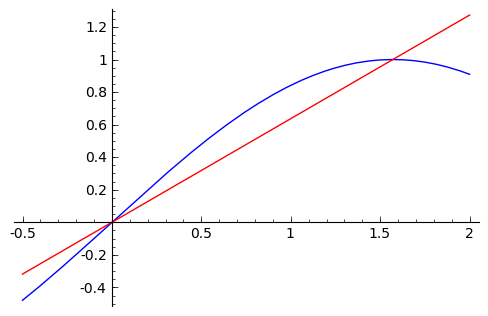
\includegraphics[width=9cm]{premiere_epreuve_exo5.png}
  \caption{La région $E$}
  \end{center}
 \end{figure}
 
\begin{equation}
  \begin{aligned}
    &\int_{E}x+2y \, dS=\int_0^{\pi/2}\int_{2x/\pi}^{\sin(x)} x+2y\, dy\,dx\\
    &=\int_0^{\pi/2}x\sin(x)-\frac{2}{\pi}x^2+\sin^2(x)-\frac{4x^2}{\pi^2}\,dx\\
    &=\int_0^{\pi/2}x\sin(x)-\frac{(2\pi+ 4)}{\pi^2}x^2+\sin^2(x)\,dx.
  \end{aligned}
\end{equation}

Cette intégrale peut être calculée en considérant un terme à la fois. D'abord on obtient
\[
\int_0^{\pi/2}x\sin(x)\,dx=\left.-x\cos(x)\right\vert_{0}^{\pi/2}+\int_0^{\pi/2}\cos(x)\,dx=1 ;
\]
et
\[
-\int_0^{\pi/2}\frac{(2\pi+ 4)}{\pi^2}x^2 \,dx=-\frac{(\pi^2+ 2\pi)}{12}.
\]
Enfin, on observe 
\[
\int_0^{\pi/2}\sin^2(x)\,dx=\left. -\cos(x)\sin(x)\right\vert_{0}^{\pi/2}+ \int_0^{\pi/2}\cos^2(x)\,dx,
\]
ce qui nous permet d'écrire
 \[
\int_0^{\pi/2}\sin^2(x)+\cos^2(x) \,dx=2 \int_0^{\pi/2}\sin^2(x)\,dx,
\]
et donc
\[
\int_0^{\pi/2}\sin^2(x)\,dx=\frac{\pi}{4}.
\]
\end{corrige}
